% SPDX-License-Identifier: Apache-2.0
\section{Lerneinheiten: vom Lernversprechen zum rekursiven Abschluss}
\label{sec:learning-units}
Der Graph sagt, welche Ziele es gibt und was sie voraussetzen. Er sagt
nicht, welche Ziele zusammen ein fachliches Ganzes bilden, das eine Person
als Thema beginnt und abschließt. Diese Aufgabe übernimmt die Lerneinheit.
Dieser Abschnitt definiert ihren Umfang, ihren abgeleiteten Abschluss und
die Grenzen von Voraussetzungen zwischen ganzen Einheiten.
Abschnitt~\ref{sec:assessment} baut darauf die implizite Beherrschung auf.

\begin{principle}{Fachliche Einheit statt Kalenderschublade}
Eine \textbf{Lerneinheit} (englisch \emph{learning unit}, künftiger
technischer Begriff \code{LearningUnit}) verbindet ein verständliches
Lernversprechen mit eigenen Lernzielen und gegebenenfalls kleineren
Lerneinheiten, ihren \emph{Kindeinheiten}. Die Struktur ist rekursiv:
Mechanik kann Kinematik und Dynamik enthalten; Kinematik kann ihrerseits
weitere Einheiten enthalten.
Schuljahr, Semester und Lernwoche sind mögliche Planungsbezüge, keine
Synonyme für eine Lerneinheit. Personalisierungsstufen 1--4, QA-Reifegrade
und das Schwierigkeitsfeld \code{level} behalten ihre bisherige Bedeutung.
\end{principle}

\subsection{Motivation und eigener fachlicher Anspruch}
\label{sec:unit-claims}
Die Einheit beantwortet zuerst: \emph{Was kann ich danach, und wozu ist
das nützlich?} Ein Motivationsauftakt macht dieses Versprechen verständlich,
bevor einzelne Aufgaben oder Ziele angeboten werden. Der Auftakt ist eine
didaktische Funktion. Wenn er als echtes Orientierungsziel modelliert ist,
gilt dessen eigener Abschlussvertrag (Abschnitt~\ref{sec:orientation}); eine
synthetische Überschrift ist dadurch kein zusätzliches Lernziel. Aus einem
abgeleiteten Abschluss folgt keine Behauptung, dass ein Motivationsgespräch
tatsächlich stattgefunden hat.

Eine größere Einheit kann gegenüber ihren Kindeinheiten drei verschiedene
Ansprüche erheben:
\begin{itemize}
\item \textbf{Zusammenfassen (Aggregat).} Die Einheit fasst vorhandene
 Kompetenzen ihrer Kinder nur zusammen. Dann braucht sie keine neue eigene
 Prüfung.
\item \textbf{Integrieren (Synthese).} Verspricht die Einheit zusätzlich die
 selbstständige Integration dieser Kompetenzen, kann eine eigene
 Syntheseprüfung diesen Anspruch prüfen. Sie kann sich dabei auf bereits
 in Kindern erworbene Kompetenzen beschränken. Für reine Synthese müssen
 keine künstlichen neuen Inhaltsziele erfunden werden. Die Rolle der
 Syntheseprüfung ist der zusätzliche Integrationsnachweis, nicht das
 erneute Bestehen aller Kinder.
\item \textbf{Eigene Fachkompetenzen.} Zusätzliche eigene Fachkompetenzen
 sind ebenfalls möglich; sie brauchen ihre eigene Erwerbszuordnung und
 gültige Prüfungsdeckung.
\end{itemize}

\subsection{Direkter Erwerb, Kinder und Gesamtumfang}
Eine autoritative, versionierte Einheit $U$ wird durch drei Größen
beschrieben:
\begin{itemize}
\item $\Own(U)$ bezeichnet die direkt zugeordneten atomaren
 \emph{Erwerbsziele}, kurz: die eigenen Ziele. Echte Orientierungs-,
 Prüfungs- und Memorierziele können dazugehören; reine Strukturmarker nicht.
\item $\Children(U)$ enthält die verpflichtenden Kindeinheiten, die
 \emph{Pflichtkinder}. Wahlentscheidungen sind zuvor aufgelöst.
\item $T(U)$ ist die eindeutige gesamte Zielmenge, der \emph{Gesamtumfang}:
\begin{equation}
 T(U)=\Own(U)\cup\bigcup_{V\in\Children(U)}T(V).
 \label{eq:unit-targets}
\end{equation}
\end{itemize}
In Abbildung~\ref{fig:recursive-unit} hat Kinematik die eigenen Ziele
$\{\nd{a},\nd{b},\nd{q_K},\nd{k_K}\}$, Dynamik $\{\nd{d},\nd{q_D}\}$ und
Mechanik nur die Syntheseprüfung $\{\nd{q_S}\}$. Der Gesamtumfang von
Mechanik umfasst alle sieben Ziele.

Für Umfang und Zuordnung gelten diese Regeln:
\begin{itemize}
\item Der aufgelöste Gesamtumfang ist nicht leer. Ein leerer
 Navigationsmarker ist keine abgeschlossene Lerneinheit. Ein Aggregat darf
 dagegen leere eigene Ziele haben, wenn seine Pflichtkinder den
 Gesamtumfang tragen.
\item Jeder Ersterwerb ist auf der kleinsten fachlich zuständigen
 autoritativen Einheit verortet. Eine Elternansicht darf dieselben
 stabilen Ziele zeigen, ohne sie erneut als eigene Erwerbsziele zu
 beanspruchen.
\item Überlappende Referenzen werden als Mengen vereint; sie erzeugen weder
 zusätzliche Ziele noch doppelte Fortschrittspunkte.
\item Die Zuordnung der eigenen Ziele und die fachlich geprüfte Bedeutung
 der eigenen Prüfungen bilden den \emph{lokalen Vertrag} der Einheit
 (Abschnitt~\ref{sec:assessment}). Ein bloßer Fokuswechsel verändert diese
 Zuordnung und den lokalen Vertrag nicht.
\item Jedes Inhaltsziel in $\Own(U)$ braucht einen eigenen lokalen
 Prüfungsverbraucher, also eine eigene Prüfung der Einheit, die es
 voraussetzt, und unabhängig geprüfte Anwendungsdeckung in Aufgabe und
 regulärem Bewertungsraster. Ohne diese Deckung ist der lokale Vertrag
 ungültig; eine zusätzliche frei gewählte Anerkennungsmaske ist kein Ersatz.
\end{itemize}

Die Einbettung benutzt die vorhandene Programm- und Platzierungsstruktur
beziehungsweise die geprüfte Kompositionssicht
(Abschnitt~\ref{sec:context-model}). Eine fachliche Einheit ist nicht allein
deshalb definiert, weil ein Cluster gerade aufgeklappt ist. Ebenso wenig
wird jeder beliebige \code{contains}-Cluster automatisch zur Lerneinheit.
Insbesondere bleibt die allgemeine Clustererfüllung aus
Abschnitt~\ref{sec:state} von der hier erklärten, ausdrücklich autorisierten
Einheitsstruktur unterschieden.

\subsection{Abschluss ohne zusätzlich gespeicherte Unit-Mastery}
Die vollständige Einheit ist abgeschlossen genau dann, wenn ihre eigenen
Ziele erfüllt und alle verpflichtenden Kinder abgeschlossen sind:
\begin{equation}
 \Complete(U)\iff
 \bigl(\Own(U)\subseteq\Meff\bigr)\ \land\
 \bigwedge_{V\in\Children(U)}\Complete(V).
 \label{eq:unit-complete}
\end{equation}
Der Abschluss wird aus den atomaren Ergebnissen abgeleitet. Es entsteht
keine gespeicherte \code{UnitMastery}, die Ergebnisse auf Kinder
zurückschreibt. Prüfungs- und Memorierziele bleiben ausschließlich
explizit. Daher kann eine bestandene Elternprüfung keine offene Kindprüfung
und keinen fehlenden verifizierten Kartenabruf ersetzen.

Für die Formen aus Abschnitt~\ref{sec:unit-claims} bedeutet das Folgendes.
Ein reines Aggregat darf ohne eigene Prüfung bestehen: Sein Abschluss folgt
aus den Kindern und eventuell anderen eigenen Pflichten. Eine Syntheseeinheit
kann dagegen eine eigene Prüfung, aber keine neuen Inhaltsziele
haben. Ihre Prüfung ist dann zusätzlich erforderlich. Eine reine Kartensammlung
begründet keinen Anspruch unabhängiger fachlicher Anwendung; ihre tatsächlichen
Abrufpflichten bleiben ausdrücklich zu erfüllen. Eine fachlich zum Kind
gehörige Abrufpflicht darf nicht allein zur Erzeugung eines Kindabschlusses
auf die Elterneinheit verschoben werden.

\begin{figure}[htbp]\centering
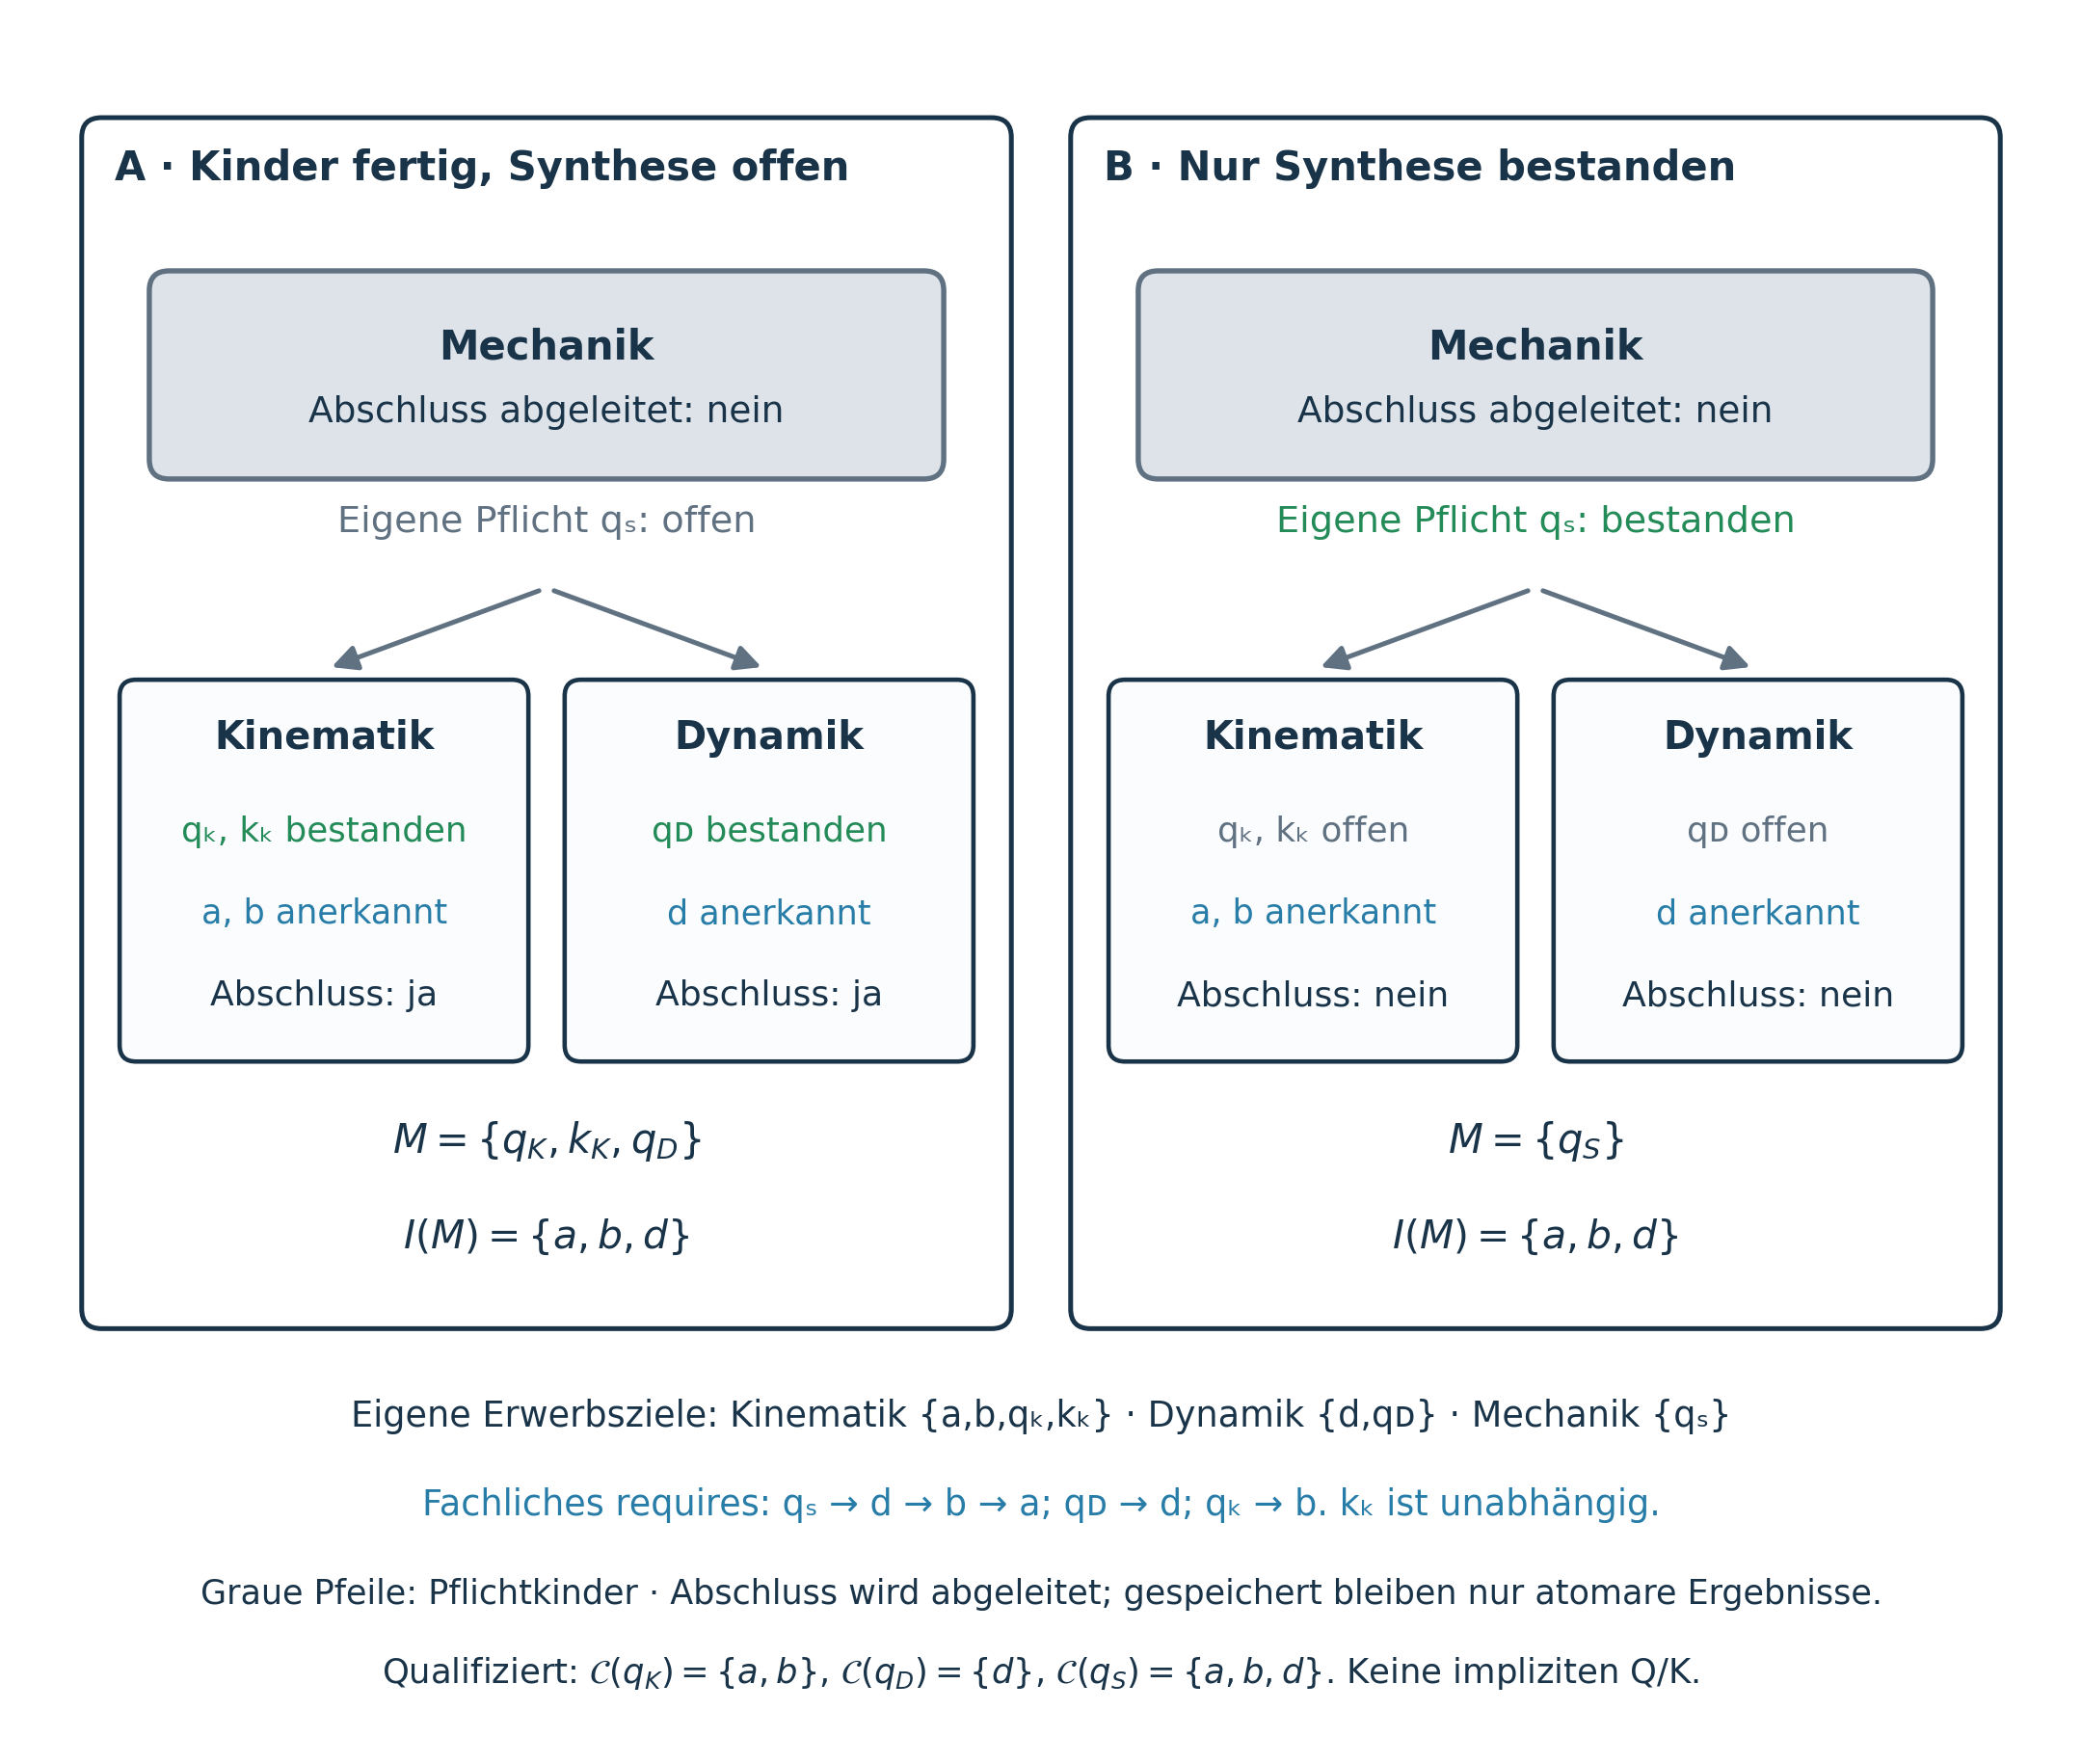
\includegraphics[width=\linewidth]{assets/graph-definition/16-recursive-learning-unit.png}
\caption[Mechanik als rekursive Lerneinheit]{Illustrative Hierarchie mit
eigenständigen Kindverträgen. Fall~A (links): Beide Kinder sind vollständig
abgeschlossen, ihre Kompetenzen global anerkannt; die offene
Syntheseprüfung \nd{q_S} hält allein den Elternabschluss offen.
Fall~B (rechts): Nur die Elternprüfung ist bestanden. Sie erzeugt keine
Kindprüfungen, keinen Kartenabruf und keine Anerkennung der
Kindkompetenzen. Graue Pfeile zeigen ausschließlich die
Einheitshierarchie; die fachlichen Kanten stehen getrennt darunter.
Im Bild sind \nd{q_K}, \nd{q_D} und \nd{q_S} Prüfungsziele, \nd{k_K} ist
ein Memorierziel, und \nd{a}, \nd{b}, \nd{d} sind Inhaltsziele.
\glqq Kind-I\grqq{} und \glqq Eltern-I\grqq{} meinen die implizite Menge
$I_U$ der jeweiligen Einheit.}
\label{fig:recursive-unit}\end{figure}
\FloatBarrier

\subsection{Anerkennung vor dem Gesamtabschluss}
Eine passende bestandene Prüfung kann die eigenen Inhaltsziele
einer Einheit anerkennen, bevor eine davon unabhängige Karte oder eine andere
Kindeinheit abgeschlossen ist. Diese Anerkennung ist global wirksam. Eine
noch offene Syntheseprüfung der Elterneinheit nimmt sie nicht zurück.

Für jede Einheit wird deshalb nur die Anerkennung ihrer \emph{eigenen}
Ziele berechnet, soweit sie keine Prüfungs- oder Memorierziele sind. Die
Elterneinheit bildet aus allen Nachfahren
keinen neuen vergrößerten Anerkennungsumfang. Sonst könnte ihre Prüfung
untergeordnete Prüfungs- oder Kartenpflichten unzulässig umgehen.
Eine Elternprüfung kann zusätzliche Integration belegen, ohne die
ursprüngliche Nachweisbedeutung der Kindverträge rückwirkend zu erweitern.
Die genaue Formel und ihre Inhaltsbedingungen stehen in
Abschnitt~\ref{sec:assessment}.

\subsection{Voraussetzungen und die Grenze einer Einheitsfolge}
Zwei Arten von Voraussetzungen sind zu unterscheiden:
\begin{itemize}
\item Ein atomarer \code{requires}-Bezug auf eine Kompetenz fordert diese
 Kompetenz. Er fordert nicht automatisch den Abschluss ihrer gesamten
 Einheit.
\item Eine \emph{Einheitsvoraussetzung} ist eine ausdrücklich autorisierte
 Voraussetzung zwischen ganzen Lerneinheiten. Sie bedeutet
 \emph{Vollabschluss} der vorausgesetzten Einheit und gehört zum
 Kompositionsvertrag außerhalb der bisherigen Grundrelationen $C$ und $R$.
\end{itemize}
Diese Aussagen dürfen weder im Compiler noch im Coach verwechselt werden.

Die Einheitshierarchie muss azyklisch sein. Wer darüber hinaus eine
ungeteilte Abschlussfolge von Einheiten behauptet, in der jede Einheit
vollständig abgeschlossen wird, bevor die nächste beginnt, muss auch deren
Voraussetzungsgraphen prüfen. Ein atomarer DAG genügt nicht: Bei
$a\to b\to c$, $\Own(U)=\{a,c\}$ und $\Own(V)=\{b\}$ braucht $U$ die
Einheit $V$ wegen $a\to b$ und $V$ die Einheit $U$ wegen $b\to c$. Nach
Zusammenfassung entsteht also eine Abhängigkeit in beide Richtungen. $U$
und $V$ sind so keine gültige ungeteilte Vollabschlussfolge. Die Diagnose
erfordert eine andere Gruppierung oder einen ausdrücklich feineren
Erwerbsablauf; sie erzeugt keine stillschweigenden Einheitssperren aus
atomaren Kanten.

Die atomare Normalform und die Migrationsreihenfolge aus
Abschnitt~\ref{sec:validity} gelten weiterhin: vollständige atomare
Voraussetzungen sichern, dadurch redundante nichtatomare Anforderungen
entfernen und erst danach die atomare Relation transitiv reduzieren.
Daraus folgt noch keine neue Minimalitätsregel für eine erst zu
beschließende Relation von Einheitsvoraussetzungen.

\begin{principle}{Zugangsprofil noch offen}
Eine fachliche Erwerbsordnung ist noch keine technische Zugangssperre.
Ob und wann eine Einheitsvoraussetzung einen harten Zugangsschutz, eine
\emph{Einheitssperre}, erzwingt, und wie dann direkte Prüfungsversuche
behandelt werden, ist \textbf{noch nicht entschieden}. Ein solches Profil
wäre gesondert zu beschließen und zu prüfen. Die Einheitendefinition führt
es nicht ein.
\end{principle}

Nur \emph{falls} später ein ausdrückliches Sperrprofil gewählt wird, könnte
man für autorisierte Vorgängereinheiten $\operatorname{Pred}(U)$ definieren:
\[
 \operatorname{Open}(U)=\bigwedge_{V\in\operatorname{Pred}(U)}
      \operatorname{Cleared}(V),\qquad
 \operatorname{Cleared}(U)=\operatorname{Open}(U)\land\Complete(U).
\]
$\Complete$ beschreibt die vorhandenen Nachweise, $\operatorname{Cleared}$
nur die bedingte Kurspolitik. Weder das Öffnen noch diese abgeleitete
Freigabe vergibt Mastery. Ob direkte Prüfungen bei geschlossenem Zugang
zulässig bleiben, entscheidet diese bloße Beispielgleichung nicht.

\sources{%
\srcref{docs/concept/skill-graph/learning-units.md}{Lerneinheiten};
\srcref{docs/concept/skill-graph/learning-unit-progression.md}{Einheitsfolge und Zugangsprofile};
\srcref{docs/concept/skill-graph/graph-definition.md}{Graph Definition, Abschnitt 12};
\srcref{docs/concept/skill-graph/assessment-gated-completion.md}{Anerkennung und globaler Abschluss}.}
